% ============================================================================
%  ARTIGO CIENTÍFICO: TRABALHO DE CONCLUSÃO DE CURSO (TCC / PFC)
%  Faculdade Engenheiro Salvador Arena (CEFSA / FESA): modelo oficial V-05
% ----------------------------------------------------------------------------
%  Este arquivo contém o conteúdo do artigo. Margens, fontes, entrelinhas,
%  recuos, cabeçalho, rodapé, notas de rodapé, legendas, fontes de figura,
%  tabela e quadro, e referências ficam na classe pfccefsa.cls.
% ============================================================================
%!TEX program = xelatex

\documentclass{pfccefsa}

\usepackage{amsmath,amssymb}
\usepackage{csquotes}
\usetikzlibrary{arrows.meta,positioning,fit,calc}
\addbibresource{referencias.bib}

% Estilo único dos diagramas TikZ.
\tikzset{
  pfcbox/.style={
    draw,
    rounded corners=1.5pt,
    align=center,
    font=\footnotesize,
    inner sep=3pt,
    minimum height=0.85cm,
    text width=2.35cm,
    execute at begin node={\spaceskip=0pt}
  },
  pfcwide/.style={pfcbox, text width=3.1cm},
  pfcsmall/.style={pfcbox, text width=1.85cm},
  pfclayer/.style={draw, rounded corners=3pt, inner sep=4pt},
  pfcarrow/.style={-{Latex[length=1.6mm]}, thick},
  pfcflow/.style={-{Latex[length=1.6mm]}, thick, dashed}
}

% ----------------------------------------------------------------------------
%  DADOS DO TRABALHO
% ----------------------------------------------------------------------------
\titulo{Caracterização reprodutível do mapa de Hénon filtrado para
comunicação: arquitetura, verificação e segurança}

\autores{Kauê de Souza Silva, Roger Freitas Pereira, Marcos Felipe Correa
Soares, Guilherme Rodrigues dos Santos\footnote{Faculdade Engenheiro Salvador
Arena, Centro Educacional da Fundação Salvador Arena, Estrada dos Alvarengas,
4001, São Bernardo do Campo, SP, Brasil}}

\orientador{Prof. Dr. Vinícius da Silva Borges}

\curso{Ciência da Computação}
\diainicial{16}
\diafinal{16}
\mes{Novembro}
\ano{2026}

\begin{document}

\imprimirtitulo
\imprimirautores
\imprimirorientador

\begin{resumo}
Este trabalho apresenta uma caracterização reprodutível do mapa de Hénon
com filtro FIR na malha de realimentação, voltada ao projeto de geradores
caóticos para comunicação. O problema combina a necessidade de limitar a
banda do sinal com o risco de o filtro destruir o regime caótico. O estudo
organiza 184 varreduras em quatro tipos de filtro e sete janelas de projeto,
classifica cada ponto pelo maior expoente de Lyapunov e reúne os resultados em
mapas de cobertura caótica. A contribuição de engenharia é uma ferramenta
modular que separa configuração, varredura, checkpoints, estatística, figuras,
números e auditoria. O desempenho foi medido em um Intel Core i7-8550U: o
kernel da varredura é 53,3 vezes mais rápido que o modo Python puro com uma
thread, a carga de 4.000 pontos ganha 3,58 vezes com oito threads em quatro
núcleos físicos, e as 184 varreduras levam 575 s. A classificação dos 4.000
pontos é idêntica com uma e com oito threads. O pipeline adota controles
fail-closed para checkpoints e para a auditoria do texto. Os resultados
mostram que o ganho DC é uma variável central e que os filtros realizados não
reproduzem exatamente a máscara nominal. As limitações incluem a classificação
local, o horizonte finito e a ausência de canais com ruído ou de garantia
criptográfica.
\end{resumo}

\palavraschave{caos. mapa de Hénon. filtros FIR. reprodutibilidade. segurança
de software.}

\begin{abstract}
This work presents a reproducible characterization of the Hénon map with an
FIR filter in the feedback loop for the design of chaotic communication
generators. The problem combines the need to limit the signal bandwidth with
the risk that the filter destroys the chaotic regime. The study organizes 184
sweeps over four filter types and seven design windows, classifies each point
by its largest Lyapunov exponent, and summarizes the results in
chaotic-coverage maps. The engineering contribution is a modular tool that
separates configuration, sweep, checkpoints, statistics, figures, manuscript
numbers, and auditing. Performance was measured on an Intel Core i7-8550U:
the sweep kernel is 53.3 times faster than pure Python with one thread, the
4,000-point load gains 3.58 times with eight threads on four physical cores,
and the 184 sweeps take 575 s. The classification of the 4,000 points is
identical with one and eight threads. The pipeline uses fail-closed controls
for checkpoints and manuscript auditing. The results show that the DC gain is
a central design variable and that the realized filters do not exactly
reproduce the nominal mask. Limitations include the local classification, the
finite horizon, and the absence of noisy channels or cryptographic
guarantees.
\end{abstract}

\keywords{chaos. Hénon map. FIR filters. reproducibility. software security.}

% ============================================================================
\section{Introdução}
% ============================================================================

Sistemas de comunicação baseados em caos (CBCS, do inglês
\emph{chaos-based communication systems}) usam sinais caóticos como
portadores de informação. Esses sinais têm espectro largo, aparência
semelhante a ruído e sensibilidade às condições iniciais, propriedades que
motivam seu uso em esquemas de comunicação e em camadas de segurança física
\cite{Baptista2021,Kaddoum2016}. O espectro largo, porém, conflita com a
largura de banda finita dos canais reais. Uma estratégia recorrente é inserir
um filtro FIR na malha de realimentação do gerador, de modo que o próprio
sinal gerado já respeite parte da máscara espectral do canal
\cite{Eisencraft2009,Fontes2016}.

O filtro resolve o problema espectral, mas cria outro: a não linearidade passa
a atuar sobre uma combinação filtrada do estado, e o comportamento caótico do
gerador pode ser preservado, alterado ou destruído. Sincronismo e caos são
requisitos independentes. Um filtro estável pode garantir a sincronização
mestre-escravo e, ao mesmo tempo, levar o gerador a uma órbita periódica ou a
uma trajetória divergente \cite{BorgesTese2026}. Por isso, cada combinação de
tipo de filtro, janela, ordem e frequência de corte precisa ser verificada
numericamente.

Estudos anteriores caracterizaram esse problema em complexidade crescente.
Borges e Eisencraft mostraram que os coeficientes de um filtro de dois
coeficientes determinam se o mapa converge para um ponto fixo, oscila
periodicamente, entra em caos ou diverge \cite{BorgesCSF2022}, e que filtros
passa-baixas de ordem crescente podem preservar ou suprimir o caos
\cite{Borges2022sbrt}. Borges \emph{et al.} mapearam os regimes do mapa com
filtro passa-baixas no plano formado pelo número de zeros e pela frequência de
corte \cite{CNMAC2023} e estenderam a análise a filtros FIR com mais
coeficientes \cite{BorgesCNSNS2024}. O artigo do JCIS consolidou essa linha em
184 varreduras, quatro tipos de filtro e sete janelas de projeto, com
552.000 pontos de grade \cite{JCISSubmetido}.

Os resultados científicos, contudo, dependem de uma cadeia computacional
confiável. Uma varredura completa envolve milhares de pontos, dezenas de
condições iniciais e milhões de iterações. Scripts frágeis, checkpoints
corrompidos, sementes não controladas, arredondamentos inconsistentes ou uma
falha silenciosa em uma figura podem transformar um resultado plausível em um
resultado errado. A contribuição deste trabalho é tratar essa cadeia como um
problema de engenharia: arquitetura modular, execução acelerada e
paralela, verificação automática, rastreabilidade dos números e segurança do
fluxo de dados.

O objetivo geral é caracterizar o mapa de Hénon filtrado e entregar uma
ferramenta reprodutível de apoio ao projeto de geradores caóticos para
comunicação. Os objetivos específicos são: (i) organizar o pipeline de
varredura, classificação, figuras e números em componentes testáveis;
(ii) medir o desempenho do núcleo computacional e da execução completa;
(iii) verificar a reprodutibilidade dos resultados e a consistência dos
números publicados; (iv) tornar explícitos os modos de falha, as decisões de
tolerância e as barreiras de segurança; e (v) discutir os limites científicos
da classificação e do sistema de comunicação estudado.

A metodologia combina a varredura numérica do mapa filtrado com uma camada de
engenharia de software. O núcleo é compilado com Numba e paralelizado com
\texttt{prange}; os checkpoints são versionados em arquivos \texttt{.npz} com
metadados JSON; as figuras e os números do artigo são derivados dos mesmos
dados; e a integração contínua executa testes, análise estática, auditoria de
dependências e compilação do manuscrito. No ambiente de teste, a execução
completa das 184 varreduras levou 575 s, e o núcleo da varredura apresentou
fator JIT de 53,3 vezes e fator de paralelismo de 3,58 vezes em uma carga de
4.000 pontos.

O texto está organizado da seguinte forma. A Seção~\ref{sec:fundamentacao}
apresenta os conceitos de caos, sincronismo, filtros FIR, expoente de
Lyapunov e computação reprodutível. A Seção~\ref{sec:metodologia} descreve o
sistema, o estimador, a arquitetura do pacote, o fluxo de dados, o desempenho
e as camadas de verificação e segurança. A Seção~\ref{sec:resultados}
discute a validação, o desempenho medido, os mapas de classificação, o sistema
de comunicação e os testes de robustez. A Seção~\ref{sec:conclusao} resume as
contribuições, as limitações e os trabalhos futuros.

% ============================================================================
\section{Referencial teórico}
\label{sec:fundamentacao}

\subsection{Caos e o mapa de Hénon}

Um sistema determinístico é sensível às condições iniciais quando trajetórias
que começam arbitrariamente próximas se separam, em média, de forma
exponencial. Essa propriedade, chamada de dependência sensível das condições
iniciais, é a marca prática do caos e limita a previsão de longo prazo mesmo
quando as equações são conhecidas \cite{Alligood1996}. O mapa de Hénon é um
exemplo bidimensional discreto e amplamente usado como gerador em estudos de
comunicação \cite{Henon1976}:
\begin{equation}
  \begin{cases}
    x_1(n+1) = \alpha - x_1^2(n) + \beta\,x_2(n),\\
    x_2(n+1) = x_1(n),
  \end{cases}
  \label{eq:henon_pfc}
\end{equation}
com $\alpha=1{,}4$ e $\beta=0{,}3$ no regime caótico canônico. Para esses
parâmetros, o mapa tem atrator estranho, órbitas periódicas imersas e regiões
de divergência no espaço de parâmetros \cite{Gallas1993}.

A Figura~\ref{fig:henon_pfc} contrasta dois comportamentos do mapa. Em
(a), duas condições iniciais separadas por $10^{-3}$ em $x_2(0)$ produzem
trajetórias que se afastam rapidamente, comportamento esperado no regime
caótico. Em (b), com $\alpha=0{,}9$, as duas trajetórias convergem para a
mesma órbita periódica. A diferença entre os dois casos não é de escala, mas
de classe dinâmica, e é exatamente essa distinção que a ferramenta precisa
automatizar.

\begin{figura}{Sinais $x_1(n)$ do mapa de Hénon para duas condições iniciais
próximas: (a) $\alpha=1{,}4$, comportamento caótico; (b) $\alpha=0{,}9$,
órbita periódica. A separação inicial é $10^{-3}$ em $x_2(0)$.}{Fonte:
Autoria própria (2026)}
  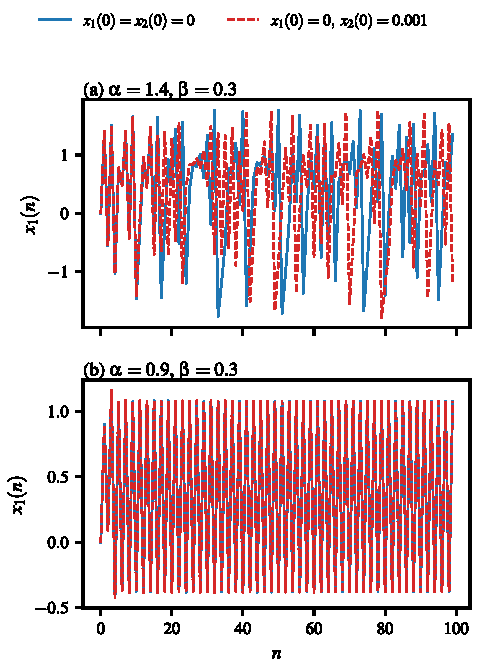
\includegraphics[width=0.45\textwidth]{figures/fig_henon_signals.pdf}
  \label{fig:henon_pfc}
\end{figura}

\subsection{Sincronismo e sistema de comunicação}

Em um CBCS coerente do tipo mestre-escravo, o transmissor contém o gerador
caótico e o receptor contém uma cópia do mesmo gerador, dirigida pelo sinal
recebido. Quando a não linearidade atua sobre uma única variável escalar, o
erro de sincronização $\mathbf{e}(n)=\hat{\mathbf{x}}(n)-\mathbf{x}(n)$ obedece
a uma recursão linear. A sincronização é atingida quando todos os
autovalores da matriz dessa recursão estão dentro do círculo unitário
\cite{Pecora1990}. Em um canal ideal, essa condição basta para o receptor
acompanhar o transmissor depois de um transiente inicial.

O transmissor usado neste trabalho codifica a mensagem $m(n)$ em
$\{-1,+1\}$ e a soma à variável caótica:
\begin{equation}
  s(n) = x_1(n) + \mu\,m(n),
  \label{eq:transmissor_pfc}
\end{equation}
com profundidade de modulação $\mu=0{,}01$. O receptor estima a mensagem pela
diferença entre o sinal recebido e o estado local depois da sincronização.
O canal pode ser ideal, que apenas copia o sinal, ou um filtro FIR
 passa-baixas que representa a largura de banda finita do meio
\cite{Eisencraft2009,Fontes2016}. As métricas usuais são a taxa de erro de
bit (BER) e o erro quadrático médio (MSE), calculados depois de descontar o
atraso de grupo do canal.

A Figura~\ref{fig:comm_pfc} resume a arquitetura. O mesmo filtro FIR é
inserido na malha do transmissor e na do receptor. Essa escolha preserva a
estabilidade da recursão de erro para qualquer filtro FIR estável, mas não
garante que o gerador continue caótico \cite{BorgesTese2026}. O filtro também
pode alterar o próprio sinal transmitido, de modo que a verificação do
gerador e a verificação do enlace são etapas distintas.

\begin{figura}{Sistema de comunicação mestre-escravo com o mesmo filtro FIR no
transmissor e no receptor. O canal pode ser ideal ou FIR.}{Fonte: Autoria
própria (2026)}
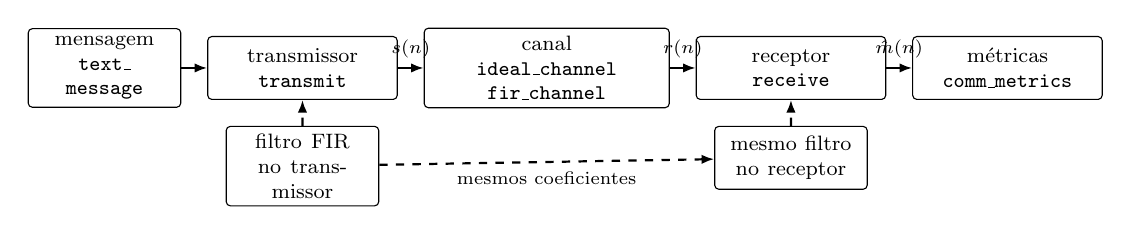
\begin{tikzpicture}[node distance=3.5mm and 3.5mm, scale=0.94, transform shape]
  \node[pfcsmall] (msg) {mensagem\\ \texttt{text\_}\\ \texttt{message}};
  \node[pfcbox, right=of msg] (tx) {transmissor\\ \texttt{transmit}};
  \node[pfcwide, right=of tx] (ch) {canal\\ \texttt{ideal\_channel}\\ \texttt{fir\_channel}};
  \node[pfcbox, right=of ch] (rx) {receptor\\ \texttt{receive}};
  \node[pfcbox, right=of rx] (met) {métricas\\ \texttt{comm\_metrics}};
  \node[pfcsmall, below=of tx] (ftx) {filtro FIR\\ no transmissor};
  \node[pfcsmall, below=of rx] (frx) {mesmo filtro\\ no receptor};
  \draw[pfcarrow] (msg) -- (tx);
  \draw[pfcarrow] (tx) -- node[above, font=\scriptsize]{$s(n)$} (ch);
  \draw[pfcarrow] (ch) -- node[above, font=\scriptsize]{$r(n)$} (rx);
  \draw[pfcarrow] (rx) -- node[above, font=\scriptsize]{$\hat{m}(n)$} (met);
  \draw[pfcflow] (ftx) -- (tx);
  \draw[pfcflow] (frx) -- (rx);
  \draw[pfcflow] (ftx) -- node[below, font=\scriptsize]{mesmos coeficientes} (frx);
\end{tikzpicture}
\label{fig:comm_pfc}
\end{figura}

Os blocos da Figura~\ref{fig:comm_pfc} correspondem aos seguintes
arquivos:
\begin{itemize}[leftmargin=1.2em,itemsep=0pt,topsep=2pt]
  \item \texttt{src/chaotic\_pfc/dynamics/signals.py}: \texttt{text\_message};
  \item \texttt{src/chaotic\_pfc/comms/transmitter.py}: \texttt{transmit};
  \item \texttt{src/chaotic\_pfc/comms/channel.py}: \texttt{ideal\_channel} e \texttt{fir\_channel};
  \item \texttt{src/chaotic\_pfc/comms/receiver.py}: \texttt{receive};
  \item \texttt{src/chaotic\_pfc/comms/metrics.py}: \texttt{comm\_metrics};
  \item \texttt{src/chaotic\_pfc/config.py}: parâmetros do sistema.
\end{itemize}

A literatura mostra que a presença de caos no sinal transmitido não deve ser
presumida. Candido \emph{et al.} mostraram que um sistema de comunicação
baseado em caos pode transmitir sinais que já não são caóticos no sentido
dinâmico \cite{Candido2015}. Fontes e Eisencraft calcularam o maior expoente
de Lyapunov do gerador filtrado em função dos coeficientes e da mensagem
\cite{Fontes2017,FontesSAI}. Este trabalho adota essa perspectiva: a
ferramenta verifica o gerador antes de atribuir qualquer desempenho ao
enlace.

\subsection{Filtro FIR, ganho DC e janelas}

Um filtro FIR de ordem $N_z$ tem $N_s=N_z+1$ coeficientes $c_k$ e resposta
ao impulso de duração finita. Sua função de transferência é
\begin{equation}
  H(z)=\sum_{k=0}^{N_z} c_k z^{-k},
  \qquad
  G=H(e^{j0})=\sum_{k=0}^{N_z} c_k,
  \label{eq:fir_pfc}
\end{equation}
em que $G$ é o ganho DC. No mapa filtrado, a não linearidade atua sobre
\begin{equation}
  x_3(n)=\sum_{k=0}^{N_z} c_k x_1(n-k),
  \qquad
  x_1(n+1)=\alpha-x_3^2(n)+\beta x_2(n).
  \label{eq:filtrado_pfc}
\end{equation}
O ponto fixo satisfaz $x_1^\star=\alpha-(G x_1^\star)^2+\beta x_1^\star$ para
$G\neq0$. Quando $G$ é próximo de zero, o ponto fixo se desloca e o mapa pode
se tornar localmente estável para qualquer escolha de coeficientes
\cite{BorgesCNSNS2024}. Por isso, o ganho DC é uma variável de projeto, e não
um detalhe de implementação.

Os coeficientes são obtidos pelo método da janela \cite{Oppenheim2009}. A
resposta ideal é truncada por uma janela de $N_s$ amostras, e a forma da
janela controla o compromisso entre a largura da faixa de transição e o nível
dos lóbulos laterais. As janelas retangular, Bartlett, Hann, Hamming,
Blackman e Blackman-Harris são casos clássicos \cite{Harris1978}. A janela de
Kaiser oferece um parâmetro contínuo $\beta_K$ que permite percorrer esse
compromisso sem mudar a ordem do filtro; para $\beta_K=0$ ela se reduz à
janela retangular \cite{Kaiser1980}.

Nas ordens estudadas, o filtro realizado não reproduz exatamente a máscara
nominal. Filtros passa-faixa e rejeita-faixa ficam mais largos do que o
projetado, e o ganho DC depende do tipo de filtro. Essa diferença é uma
limitação científica, não um erro de implementação, e deve ser considerada ao
interpretar os mapas de classificação.

\subsection{Expoente de Lyapunov}

A taxa média de separação de órbitas próximas é quantificada pelo maior
expoente de Lyapunov. Para um mapa $\mathbf{x}(n+1)=\mathbf{F}(\mathbf{x}(n))$
com jacobiano $\mathbf{J}(n)$, o expoente é
\begin{equation}
  \lambda_1
  =
  \lim_{N\to\infty}\frac{1}{N}
  \sum_{n=0}^{N-1}
  \ln\left\|\mathbf{J}(n)\,\mathbf{v}(n)\right\|,
  \label{eq:lyap_pfc}
\end{equation}
com renormalização periódica do vetor tangente $\mathbf{v}(n)$ para evitar
estouro numérico. O método da matriz tangente e a ortogonalização de
Gram-Schmidt calculam o espectro completo \cite{Benettin1980a,Benettin1980b}.
Na prática, usa-se uma estimativa de tempo finito com um número limitado de
iterações e um limiar de decisão, e não o limite assintótico
\cite{Wolf1985,Sprott2003}.

Neste trabalho, um ponto é classificado como divergente quando a órbita deixa
a região limitada, como caótico quando a estimativa de $\lambda_1$ supera
$5\times10^{-3}$ e como não caótico caso contrário. O limiar é uma decisão
operacional, não uma fronteira matemática exata. A classificação é local no
plano de parâmetros e depende do horizonte de integração, do número de
condições iniciais e do critério de parada.

\subsection{Computação científica reprodutível}

Uma varredura completa combina milhares de pontos de grade, dezenas de
condições iniciais e milhões de iterações. A reprodutibilidade exige que a
mesma semente, a mesma versão do código e o mesmo ambiente produzam os mesmos
resultados. Isso é particularmente delicado quando o núcleo é compilado e
paralelizado. Numba traduz funções Python para código de máquina e permite
paralelismo com \texttt{prange} \cite{Lam2015}; NumPy e SciPy fornecem as
operações vetoriais e o projeto dos filtros \cite{Harris2020,Virtanen2020}.
Testes baseados em propriedades complementam os testes de exemplo ao gerar
entradas aleatórias e verificar invariantes \cite{MacIver2019}.

A reprodutibilidade também depende da rastreabilidade dos artefatos. O
pacote \texttt{chaotic-pfc} \cite{chaoticPFC2026} organiza a configuração, a
varredura, os checkpoints, as figuras, os números do manuscrito e a auditoria
em uma única cadeia. O artigo do JCIS usa essa cadeia para produzir os 184
checkpoints e os números publicados \cite{JCISSubmetido}. O presente trabalho
discute a engenharia dessa cadeia, os seus modos de falha e as barreiras que
impedem que uma falha silenciosa chegue ao texto.

% ============================================================================
\section{Metodologia}
\label{sec:metodologia}

\subsection{Sistema estudado e grade de varredura}

O sistema estudado é o mapa de Hénon com um filtro FIR na malha de
realimentação, descrito por \eqref{eq:filtrado_pfc}. A varredura combina
quatro tipos de filtro (passa-baixas, passa-altas, passa-faixa e
rejeita-faixa) com sete janelas de projeto (retangular, Bartlett, Hann,
Hamming, Blackman, Blackman-Harris e Kaiser). Para passa-baixas e
passa-altas, a frequência de corte $\omega_c/\pi$ é o parâmetro de projeto;
para passa-faixa e rejeita-faixa, ela é o centro de uma banda de largura
nominal $\Delta\omega=0{,}05\pi$. A banda é recortada perto das bordas do
intervalo $(0,1)$, o que produz filtros assimétricos nas extremidades da
grade.

Nas seis janelas fixas, a ordem $N_z$ varia de 1 a 40 nos filtros
passa-baixas e passa-faixa e assume apenas valores pares nos filtros
passa-altas e rejeita-faixa, por causa da restrição de paridade do método da
janela. Cada configuração tem 4.000 pontos nos dois primeiros casos e 2.000
nos dois últimos. A janela de Kaiser é varrida em 40 valores de
$\beta_K\in[0{,}5,20]$, com passo $0{,}5$, para cada tipo de filtro. O
resultado é um conjunto de 184 varreduras e 552.000 pontos de grade
\cite{JCISSubmetido}.

A escolha de uma grade regular permite comparar projetos e reproduzir os
mapas, mas não representa todo o espaço de parâmetros. Em particular, a
largura de banda é fixa, a ordem máxima é 40 e os parâmetros do mapa são
$(\alpha,\beta)=(1{,}4,0{,}3)$. A Seção~\ref{sec:resultados} discute como
essas escolhas limitam a generalização dos resultados.

\subsection{Estimador e classificação}

Para cada ponto da grade, o estimador usa 25 condições iniciais em um
hipercubo de lado $0{,}1$ com um vértice no ponto fixo positivo. Cada
condição inicial passa por 500 iterações de burn-in, e o expoente é
acumulado por até 3.000 iterações. A ortogonalização modified Gram-Schmidt
(MGS) mantém o vetor tangente normalizado e evita estouro numérico. Pontos
cuja estimativa fica a menos de $5\times10^{-3}$ do limiar são recomputados
com o espectro completo, e o maior expoente resultante é o valor atribuído
ao ponto. A parada antecipada é opcional e, quando habilitada, usa
$N_{\text{map,min}}=500$ e tolerância $10^{-3}$.

A classificação tem três classes. Um ponto é divergente quando a órbita deixa
a região limitada, caótico quando a média de $\lambda_1$ sobre as condições
iniciais supera $\theta=5\times10^{-3}$ e não caótico caso contrário. A
Figura~\ref{fig:estimador_pfc} resume o fluxo. O limiar é uma decisão
operacional sobre uma estimativa de tempo finito; ele não substitui a análise
assintótica e não deve ser interpretado como uma fronteira exata.

\begin{figura}{Fluxo do estimador e da classificação. O teste de proximidade
do limiar decide se o ponto precisa de recomputação com o espectro completo.}
{Fonte: Autoria própria (2026)}
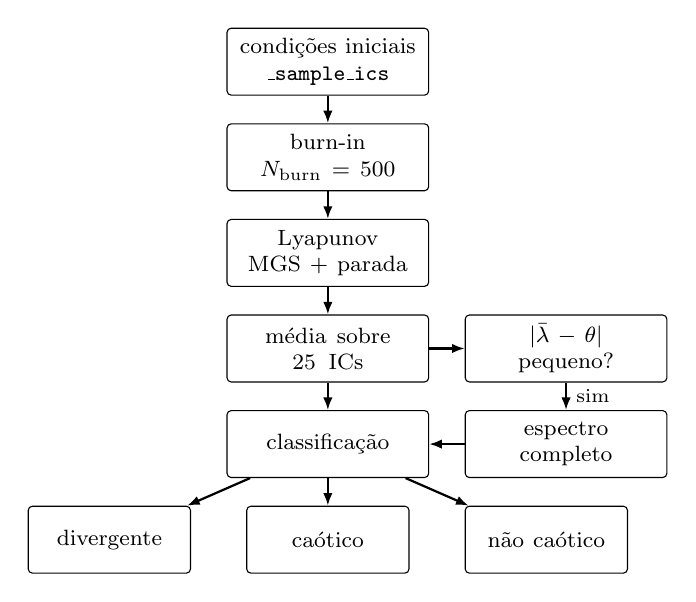
\begin{tikzpicture}[node distance=3.5mm and 4.5mm]
  \node[pfcbox] (ic) {condições iniciais\\ \texttt{\_sample\_ics}};
  \node[pfcbox, below=of ic] (burn) {burn-in\\ $N_{\text{burn}}=500$};
  \node[pfcbox, below=of burn] (lyap) {Lyapunov\\ MGS + parada};
  \node[pfcbox, below=of lyap] (mean) {média sobre\\ 25 ICs};
  \node[pfcbox, right=of mean] (dec) {$|\bar\lambda-\theta|$\\ pequeno?};
  \node[pfcbox, below=of dec] (full) {espectro\\ completo};
  \node[pfcbox, below=of mean] (class) {classificação};
  \node[pfcsmall, below left=of class] (div) {divergente};
  \node[pfcsmall, below=of class] (chaos) {caótico};
  \node[pfcsmall, below right=of class] (non) {não caótico};
  \draw[pfcarrow] (ic) -- (burn);
  \draw[pfcarrow] (burn) -- (lyap);
  \draw[pfcarrow] (lyap) -- (mean);
  \draw[pfcarrow] (mean) -- (dec);
  \draw[pfcarrow] (dec) -- node[right, font=\scriptsize]{sim} (full);
  \draw[pfcarrow] (full) -- (class);
  \draw[pfcarrow] (mean) -- (class);
  \draw[pfcarrow] (class) -- (div);
  \draw[pfcarrow] (class) -- (chaos);
  \draw[pfcarrow] (class) -- (non);
\end{tikzpicture}
\label{fig:estimador_pfc}
\end{figura}

Os blocos da Figura~\ref{fig:estimador_pfc} correspondem aos seguintes
arquivos:
\begin{itemize}[leftmargin=1.2em,itemsep=0pt,topsep=2pt]
  \item \texttt{src/chaotic\_pfc/dynamics/lyapunov.py}: \texttt{\_sample\_ics};
  \item \texttt{src/chaotic\_pfc/analysis/sweep/\_kernel.py}: \texttt{\_burn\_in\_n12} e \texttt{\_burn\_in\_nN};
  \item \texttt{src/chaotic\_pfc/analysis/sweep/\_kernel.py}: \texttt{\_lyap\_online\_core};
  \item \texttt{src/chaotic\_pfc/analysis/sweep/\_kernel.py}: \texttt{\_adaptive\_checkpoint};
  \item \texttt{src/chaotic\_pfc/analysis/sweep/\_kernel.py}: \texttt{\_samples\_summary};
  \item \texttt{src/chaotic\_pfc/analysis/sweep\_plotting/\_common.py}: \texttt{classify};
  \item \texttt{src/chaotic\_pfc/analysis/sweep/\_types.py}: limiar de classificação.
\end{itemize}

\subsection{Arquitetura do pacote}

O pacote \texttt{chaotic-pfc} é organizado em camadas. A camada de
configuração concentra os parâmetros em dataclasses e em um único
\texttt{DEFAULT\_CONFIG}. A camada de dinâmica contém o mapa, o estimador de
Lyapunov, as janelas e os sinais. A camada de comunicação contém transmissor,
canal, receptor e métricas. A camada de análise contém a varredura, os
checkpoints, a estatística e as figuras. A camada de manuscrito contém os
números, a auditoria e o PDF. A interface de linha de comando orquestra as
etapas.

A Figura~\ref{fig:arquitetura_pfc} funde a arquitetura de componentes com o
fluxo de dados até o PDF. As caixas superiores recebem a configuração e a
chamada da linha de comando. A varredura chama o kernel compilado e grava um
checkpoint. A análise lê o checkpoint e produz estatísticas, números e
figuras. A auditoria verifica o texto e os números, e a compilação produz o
PDF. As setas entre camadas mostram que cada etapa depende do artefato da
etapa anterior, e não de estado global implícito.

\begin{figura}{Arquitetura em camadas do pacote e fluxo de dados da
configuração ao PDF.}{Fonte: Autoria própria (2026)}
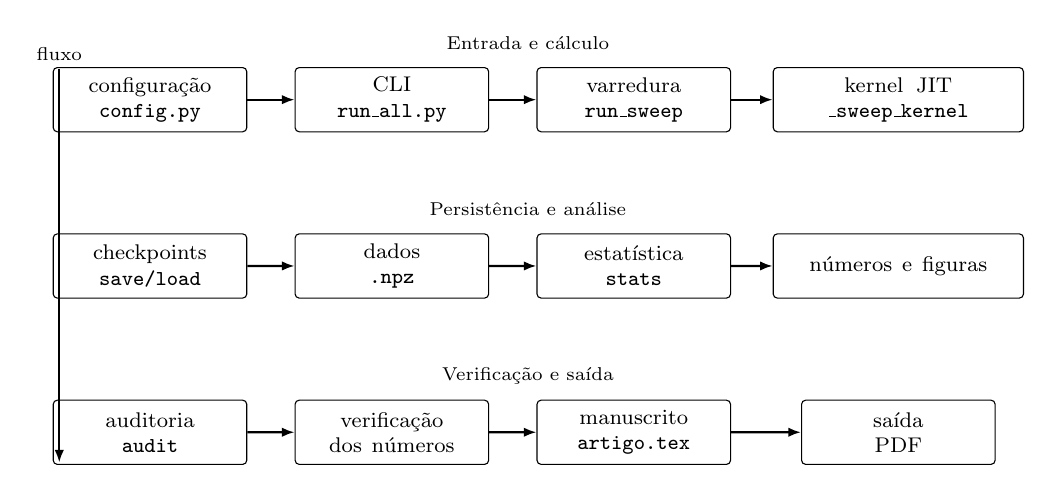
\begin{tikzpicture}[scale=0.96, transform shape]
  \node[font=\scriptsize] at (5.0,0.75) {Entrada e cálculo};
  \node[pfcbox] (cfg) at (0,0) {configuração\\ \texttt{config.py}};
  \node[pfcbox] (cli) at (3.2,0) {CLI\\ \texttt{run\_all.py}};
  \node[pfcbox] (sweep) at (6.4,0) {varredura\\ \texttt{run\_sweep}};
  \node[pfcwide] (kernel) at (9.9,0) {kernel JIT\\ \texttt{\_sweep\_kernel}};
  \draw[pfcarrow] (cfg) -- (cli);
  \draw[pfcarrow] (cli) -- (sweep);
  \draw[pfcarrow] (sweep) -- (kernel);

  \node[font=\scriptsize] at (5.0,-1.45) {Persistência e análise};
  \node[pfcbox] (io) at (0,-2.2) {checkpoints\\ \texttt{save/load}};
  \node[pfcbox] (npz) at (3.2,-2.2) {dados\\ \texttt{.npz}};
  \node[pfcbox] (stats) at (6.4,-2.2) {estatística\\ \texttt{stats}};
  \node[pfcwide] (out) at (9.9,-2.2) {números e figuras};
  \draw[pfcarrow] (io) -- (npz);
  \draw[pfcarrow] (npz) -- (stats);
  \draw[pfcarrow] (stats) -- (out);

  \node[font=\scriptsize] at (5.0,-3.65) {Verificação e saída};
  \node[pfcbox] (audit) at (0,-4.4) {auditoria\\ \texttt{audit}};
  \node[pfcbox] (check) at (3.2,-4.4) {verificação\\ dos números};
  \node[pfcbox] (tex) at (6.4,-4.4) {manuscrito\\ \texttt{artigo.tex}};
  \node[pfcbox] (pdf) at (9.9,-4.4) {saída\\ PDF};
  \draw[pfcarrow] (audit) -- (check);
  \draw[pfcarrow] (check) -- (tex);
  \draw[pfcarrow] (tex) -- (pdf);

  \draw[pfcarrow] (-1.2,0.4) -- (-1.2,-4.8);
  \node[font=\scriptsize, above] at (-1.2,0.4) {fluxo};
\end{tikzpicture}
\label{fig:arquitetura_pfc}
\end{figura}

Os blocos da Figura~\ref{fig:arquitetura_pfc} correspondem aos seguintes
arquivos:
\begin{itemize}[leftmargin=1.2em,itemsep=0pt,topsep=2pt]
  \item \texttt{src/chaotic\_pfc/config.py}: configuração;
  \item \texttt{src/chaotic\_pfc/cli/run\_all.py}: linha de comando;
  \item \texttt{src/chaotic\_pfc/analysis/sweep/\_orchestration.py}: \texttt{run\_sweep};
  \item \texttt{src/chaotic\_pfc/analysis/sweep/\_kernel.py}: \texttt{\_sweep\_kernel};
  \item \texttt{src/chaotic\_pfc/analysis/sweep/\_io.py}: \texttt{save\_sweep} e \texttt{load\_sweep};
  \item \texttt{src/chaotic\_pfc/analysis/stats/}: estatística;
  \item \texttt{src/chaotic\_pfc/paper/numbers.py}: \texttt{compute};
  \item \texttt{src/chaotic\_pfc/paper/figures.py}: figuras;
  \item \texttt{src/chaotic\_pfc/paper/audit.py}: \texttt{run\_checks};
  \item \texttt{articles/pfc/tools/} e \texttt{articles/pfc/artigo.tex}: verificação e manuscrito.
\end{itemize}

\subsection{Checkpoints, determinismo e rastreabilidade}

Cada varredura é gravada em um arquivo \texttt{.npz} com a matriz de
expoentes, o desvio, a grade de ordens, a grade de cortes e um campo de
metadados JSON. Os metadados incluem a janela, o tipo de filtro, o valor de
$\beta_K$, os parâmetros do mapa, a semente, o número de condições iniciais,
o horizonte e a política de classificação. O carregamento usa
\texttt{allow\_pickle=False}; metadados legados só são desserializados depois
de uma verificação SHA-256 contra um conjunto de digests compilado no pacote.
Essa escolha impede que um arquivo hostil execute código durante a abertura
de um checkpoint.

A semente é fixa e as perturbações são geradas antes da chamada do kernel.
O kernel distribui os pontos da grade em uma única região \texttt{prange},
com uma ordem de tarefas intercalada para equilibrar ordens leves e pesadas.
O resultado é determinístico para o mesmo número de threads e para o mesmo
ambiente. A verificação de determinismo compara as classes de todos os 4.000
pontos de uma varredura executada com uma e com oito threads; as classes são
idênticas.

\subsection{Desempenho}

As medições usam um Intel Core i7-8550U, com 4 núcleos físicos e 8 threads
lógicas, 31,1 GiB de RAM, governador \texttt{powersave}, Python 3.14.8,
NumPy 2.5.2, SciPy 1.18.0 e Numba 0.67.0. O protocolo aquece o kernel antes
das medições, executa cinco repetições para as cargas curtas e três para a
carga de 4.000 pontos, e registra a mediana e o intervalo interquartil.

A carga \texttt{mini\_sweep\_30\_points} mede o fator JIT: o modo Python puro
é 53,3 vezes mais lento que o modo Numba com uma thread. A carga
\texttt{sweep\_lowpass\_hamming\_4000} mede o paralelismo: com uma thread ela
leva 11,24 s e, com oito threads, 3,14 s, um fator de 3,58 vezes. A execução
completa das 184 varreduras, com parada antecipada, leva 575 s, ou 9,59 min.
Apenas o kernel da varredura é compilado; as cargas de mapa, Lyapunov e
pré-cálculo do banco de filtros são NumPy/Python ou SciPy e ficam próximas de
1,0 nas duas versões. A Tabela~\ref{tab:desempenho_pfc} resume.

\begin{tabela}{Medições de desempenho no i7-8550U com oito threads.}{Fonte:
Autoria própria (2026)}
\begin{tabular}[t]{lccc}
\hline
\textbf{Medida} & \textbf{Configuração} & \textbf{Resultado} & \textbf{Repetições} \\
\hline
Fator JIT & \texttt{mini\_sweep}, 1 thread & 53,3x & 5 \\
Fator de paralelismo & lowpass Hamming, 4.000 pontos & 3,58x & 3 \\
Varredura completa & 184 varreduras, 8 threads & 575 s & 1 \\
Determinismo & classes com 1 e 8 threads & idênticas & 1 \\
\hline
\end{tabular}
\label{tab:desempenho_pfc}
\end{tabela}

\subsection{Verificação e reprodutibilidade}

A verificação combina testes unitários, testes baseados em propriedades,
testes de contrato, testes metamórficos, arquivos de referência e testes de
regressão numérica. Os testes de contrato verificam que funções públicas
aceitam entradas válidas ou falham com uma exceção de domínio explícita. Os
testes metamórficos usam identidades independentes, como
$\lambda_1+\lambda_2=\ln|\beta|$ e a soma do espectro, para detectar erros que
uma comparação com um único valor de referência não revelaria. Os testes de
regressão executam o kernel e comparam os checkpoints bit a bit.

A auditoria do JCIS verifica chaves de citação, presença de DOI, estrutura,
log de compilação, idioma das figuras, tabelas e números do texto. A falha de
uma checagem é tratada como erro, e não como aviso. O PFC usa a mesma ideia
em dois scripts próprios: um extrai os números do PDF, normaliza vírgula
decimal e ponto de milhar, e confere cada valor contra os números calculados
ou contra o arquivo de medições; outro verifica se cada caminho e nome citado
nos diagramas existe no repositório. A compilação do PDF é feita com XeLaTeX
e biber, e a integração contínua executa os testes, a análise estática e a
compilação do manuscrito.

\subsection{Robustez e segurança}

O projeto adota uma postura \emph{fail-closed} nos pontos que alimentam o
texto. Se uma checagem da auditoria levanta uma exceção, o resultado é
\texttt{ERROR}, com o nome da checagem e um traceback resumido. Se um
checkpoint está corrompido, o caminho de figuras e números do artigo
interrompe a execução; o modo tolerante existe apenas para uso interativo
explícito. Esses dois casos foram encontrados durante a revisão e são
exemplos de falhas que antes poderiam passar como aviso.

As entradas públicas são validadas na borda. Parâmetros não finitos,
intervalos inválidos, ordens não inteiras, vetores com forma incompatível e
políticas de divergência desconhecidas levantam exceções específicas. A
política de divergência é explícita: \texttt{nan}, \texttt{warn} ou
\texttt{raise}. O carregamento de checkpoints verifica a integridade antes da
confiança e não lê manifestos externos em tempo de execução. A integração
contínua fixa as ações por SHA, usa permissões mínimas e executa verificações
de estilo, tipos, testes, contratos, warnings, baseline, números, PDF,
dependências, segredos e workflows. O Quadro~\ref{qua:ci_pfc} lista as
ferramentas e os jobs correspondentes.

Alguns tratamentos tolerantes são decisões conscientes. A sonda de LaTeX
retorna um fallback quando o ambiente não tem LaTeX, sem afetar resultados
científicos. A borda da CLI imprime uma mensagem e retorna código 1, em vez de
expor um traceback, mas permite \texttt{--debug}. Metadados legados
corrompidos são descartados com aviso depois da verificação de integridade.
Nenhum desses casos é um \texttt{except: pass}; a regra de análise estática
barra esse padrão.

A Figura~\ref{fig:ci_pfc} resume os portões da integração contínua. O
Quadro~\ref{qua:ci_pfc} detalha as ferramentas e o que cada uma barra. A
segurança aqui é a segurança do artefato de software e da cadeia de
ferramentas, não uma garantia criptográfica do esquema de comunicação. O
esquema de Pecora-Carroll não substitui TLS, cifras autenticadas ou
gerenciamento de chaves.

\begin{figura}{Portões da integração contínua. Cada caixa indica o job e o
tipo de falha que ele impede de avançar.}{Fonte: Autoria própria (2026)}
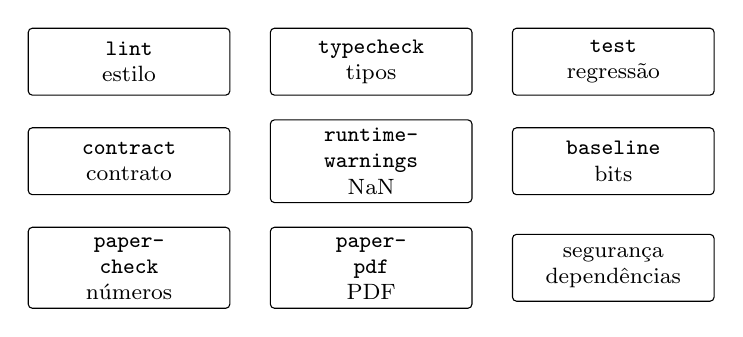
\begin{tikzpicture}[node distance=4mm and 5mm]
  \node[pfcbox] (lint) {\texttt{lint}\\ estilo};
  \node[pfcbox, right=of lint] (type) {\texttt{typecheck}\\ tipos};
  \node[pfcbox, right=of type] (test) {\texttt{test}\\ regressão};
  \node[pfcbox, below=of lint] (contract) {\texttt{contract}\\ contrato};
  \node[pfcbox, right=of contract] (warn) {\texttt{runtime-}\\ \texttt{warnings}\\ NaN};
  \node[pfcbox, right=of warn] (base) {\texttt{baseline}\\ bits};
  \node[pfcbox, below=of contract] (paper) {\texttt{paper-}\\ \texttt{check}\\ números};
  \node[pfcbox, right=of paper] (pdf) {\texttt{paper-}\\ \texttt{pdf}\\ PDF};
  \node[pfcbox, right=of pdf] (sec) {segurança\\ dependências};
\end{tikzpicture}
\label{fig:ci_pfc}
\end{figura}

\begin{quadro}{Ferramentas de integração contínua e o que cada uma barra.}
{Fonte: Autoria própria (2026)}
\begin{tabular}[t]{|p{90bp}|p{165bp}|p{115bp}|}
\hline
\textbf{Ferramenta} & \textbf{O que barra} & \textbf{Job} \\
\hline
Ruff & estilo e imports & \texttt{lint} \\
mypy & tipos & \texttt{typecheck} \\
pytest & regressão & \texttt{test} \\
Hypothesis & invariantes & \texttt{contract} \\
Semgrep & padrões de risco & \texttt{semgrep} \\
pip-audit & vulnerabilidades & \texttt{pip-audit} \\
gitleaks & segredos & \texttt{gitleaks} \\
zizmor & workflows & \texttt{zizmor} \\
CodeQL & segurança & CodeQL \\
Dependabot & dependências & Dependabot \\
\hline
\end{tabular}
\label{qua:ci_pfc}
\end{quadro}

% ============================================================================
\section{Resultados e discussão}
\label{sec:resultados}

\subsection{Validação do estimador}

O estimador foi validado no mapa sem filtro, com $\alpha=1{,}4$ e
$\beta=0{,}3$, para o qual a literatura reporta $\lambda_1=0{,}4192$
\cite{Sprott2003}. O estimador de espectro completo, com parada antecipada
desativada, produziu $\bar{\lambda}_1=0{,}4185$, cerca de 0,18\% abaixo da
referência. A identidade $\lambda_1+\lambda_2=\ln|\beta|$ foi satisfeita
dentro de $5{,}4\times10^{-9}$, o que verifica a implementação
independentemente do valor de referência. O caminho de vetor único usado nas
varreduras, com renormalização a cada dez iterações e parada antecipada,
produziu $\bar{\lambda}_1=0{,}4194$, uma diferença de 0,21\% em relação ao
espectro completo e de 0,03\% em relação à referência. As três estimativas
estão muito abaixo do limiar de $5\times10^{-3}$ usado na classificação, de
modo que o erro numérico não muda a classe dos pontos validados.

A validação não prova que todos os pontos da grade estão corretos. Ela mostra
que o estimador implementa a definição e que a identidade analítica é
respeitada. A concordância com a literatura é uma verificação independente
do código, e a identidade é uma verificação independente da literatura
\cite{Wolf1985,Benettin1980a,Benettin1980b}.

\subsection{Desempenho medido}

A Tabela~\ref{tab:desempenho_pfc} mostra que o ganho de desempenho está
concentrado no kernel da varredura. A carga de 30 pontos mede o efeito da
compilação com uma thread: o modo Python puro é 53,3 vezes mais lento. A
carga canônica de 4.000 pontos mede o efeito das threads: uma thread leva
11,24 s e oito threads levam 3,14 s, um fator de 3,58. A execução completa
das 184 varreduras leva 575 s, ou 9,59 min, com parada antecipada.

O fator de paralelismo é inferior ao número de núcleos físicos porque a carga
tem pontos leves e pesados, porque o escalonamento e a redução têm custo fixo
e porque o \texttt{prange} não garante eficiência linear. O valor de 3,58
vezes é uma medição, não uma promessa de escalabilidade. A classificação dos
4.000 pontos é idêntica com uma e com oito threads, o que indica que o
paralelismo não alterou o resultado científico dessa carga.

As cargas de mapa, Lyapunov e pré-cálculo do banco de filtros não passam pelo
kernel compilado e ficaram próximas de 1,0. Isso é esperado: o ganho de 53,3
vezes se aplica ao kernel da varredura, não a toda a biblioteca. A afirmação
de desempenho do texto é, portanto, específica e rastreável ao JSON de
medição.

\subsection{Mapas de classificação e ganho DC}

A Figura~\ref{fig:mapas_pfc} mostra os mapas de classificação para os filtros
passa-baixas e passa-altas. No passa-baixas, o caos fica abaixo de uma
fronteira que diminui com $N_z$, e a divergência aparece acima dela. No
passa-altas, o caos se concentra em baixas frequências de corte para
$N_z\ge6$ e também em frequências altas para $N_z=4$, onde a resposta do
filtro é mais permissiva. Em ordens altas, os dois filtros só são caóticos em
frequências de corte baixas.

A diferença entre os dois mapas é coerente com o ganho DC. Filtros
passa-baixas e rejeita-faixa têm $G\approx1$ e preservam a componente
contínua; filtros passa-altas e passa-faixa têm $G\approx0$ e removem essa
componente. Como o ponto fixo do mapa filtrado depende de $G$, o passa-altas
desloca o ponto fixo e torna a região caótica mais estreita. O mapa do
passa-altas é, nesse sentido, uma ilustração do efeito do ganho DC, e não uma
afirmação de que o filtro realizado tenha a máscara nominal.

Os mapas são locais: cada célula representa uma combinação de ordem e corte,
não uma região contínua. A classificação depende do limiar, do horizonte de
integração, do número de condições iniciais e da política de divergência. A
comparação entre filtros é válida dentro da grade estudada, mas não deve ser
extrapolada para ordens ou larguras de banda fora dela. Além disso, o filtro
realizado não reproduz exatamente a máscara nominal nas ordens estudadas, o
que já aparece na própria definição do projeto.

A leitura dos mapas deve separar duas questões. A primeira é onde o gerador
permanece caótico; a segunda é qual máscara o filtro realiza. No passa-baixas,
a fronteira de caos é ampla e o ganho DC é próximo de um. No passa-altas, a
região caótica é estreita e se desloca para cortes baixos. Essa assimetria é
o resultado do ganho DC e da ordem do filtro, não de uma diferença de janela.
A comparação entre os painéis usa a mesma escala de cores e a mesma grade.

\begin{figura}{Mapas de classificação no plano $(N_z,\omega_c/\pi)$ para os
filtros (a) passa-baixas com janela de Kaiser ($\beta_K=17$) e (b) passa-altas
com janela de Kaiser ($\beta_K=15{,}5$). Caótico em vermelho, não caótico em
azul e divergente em cinza.}{Fonte: Autoria própria (2026)}
\begin{minipage}[t]{0.48\textwidth}
  \centering
  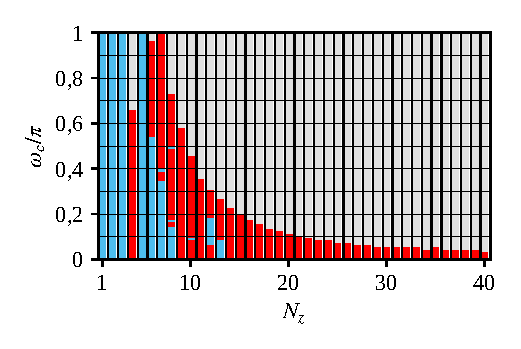
\includegraphics[width=\linewidth]{figures/kaiser_b17p0_lowpass_classification_interleaved.pdf}\\
  (a) passa-baixas
\end{minipage}\hfill
\begin{minipage}[t]{0.48\textwidth}
  \centering
  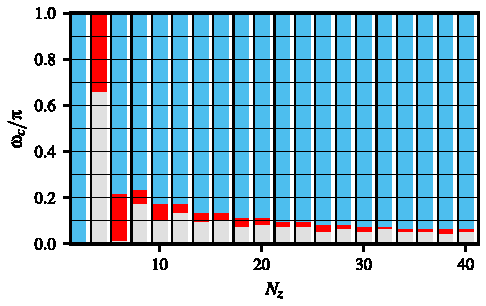
\includegraphics[width=\linewidth]{figures/kaiser_b15p5_highpass_classification_interleaved.pdf}\\
  (b) passa-altas
\end{minipage}
\label{fig:mapas_pfc}
\end{figura}

A Tabela~\ref{tab:melhores_pfc} resume a melhor configuração de cada tipo.
O passa-baixas com Kaiser $\beta_K=17$ tem a maior cobertura absoluta,
16,4\%, seguido pelo passa-faixa com Kaiser $\beta_K=15{,}5$, 7,8\%, pelo
rejeita-faixa retangular, 5,9\%, e pelo passa-altas com Kaiser
$\beta_K=15{,}5$, 5,1\%. A ordem não deve ser lida como uma ordem de
qualidade para uma aplicação específica: a escolha depende da banda do canal,
do ganho DC desejado e do custo de implementação.

\begin{tabela}{Melhor configuração de cada tipo de filtro, por cobertura
absoluta.}{Fonte: Autoria própria (2026)}
\begin{tabular}[t]{lccc}
\hline
\textbf{Tipo} & \textbf{Janela} & \textbf{$N_c$} & \textbf{$\rho_c^{\mathrm{abs}}$ (\%)} \\
\hline
Passa-baixas & Kaiser, $\beta_K=17{,}0$ & 654 & 16,4 \\
Passa-altas & Kaiser, $\beta_K=15{,}5$ & 102 & 5,1 \\
Passa-faixa & Kaiser, $\beta_K=15{,}5$ & 310 & 7,8 \\
Rejeita-faixa & Retangular & 118 & 5,9 \\
\hline
\end{tabular}
\label{tab:melhores_pfc}
\end{tabela}

\subsection{Sistema de comunicação}

A Figura~\ref{fig:comm_ideal_pfc} mostra o enlace pelo canal ideal. A
mensagem binária é recuperada sem erro, com MSE de
$8{,}7\times10^{-31}$, isto é, precisão de máquina. Esse resultado estabelece
o limite superior do sistema: quando o canal não distorce o sinal e o
receptor usa o mesmo gerador, a sincronização não é o gargalo.

O canal ideal serve como controle. Ele isola o receptor e o transmissor do
canal, de modo que qualquer erro observado pode ser atribuído à sincronização
ou à demodulação. A Figura~\ref{fig:comm_ideal_pfc} mostra os sinais no
domínio do tempo e as densidades espectrais. A mensagem recuperada segue a
mensagem original depois do transiente, e o espectro recuperado acompanha o
espectro da mensagem. O MSE é limitado pela precisão de máquina, e a BER é
zero.

\begin{figura}{Comunicação pelo canal ideal: (a) mensagem, (b) sinal
transmitido, (c) sinal recebido e (d) mensagem recuperada, com as respectivas
densidades espectrais à direita. $N=10^6$, $\mu=0{,}01$, texto ``hello'' e 20
amostras por bit.}{Fonte: Autoria própria (2026)}
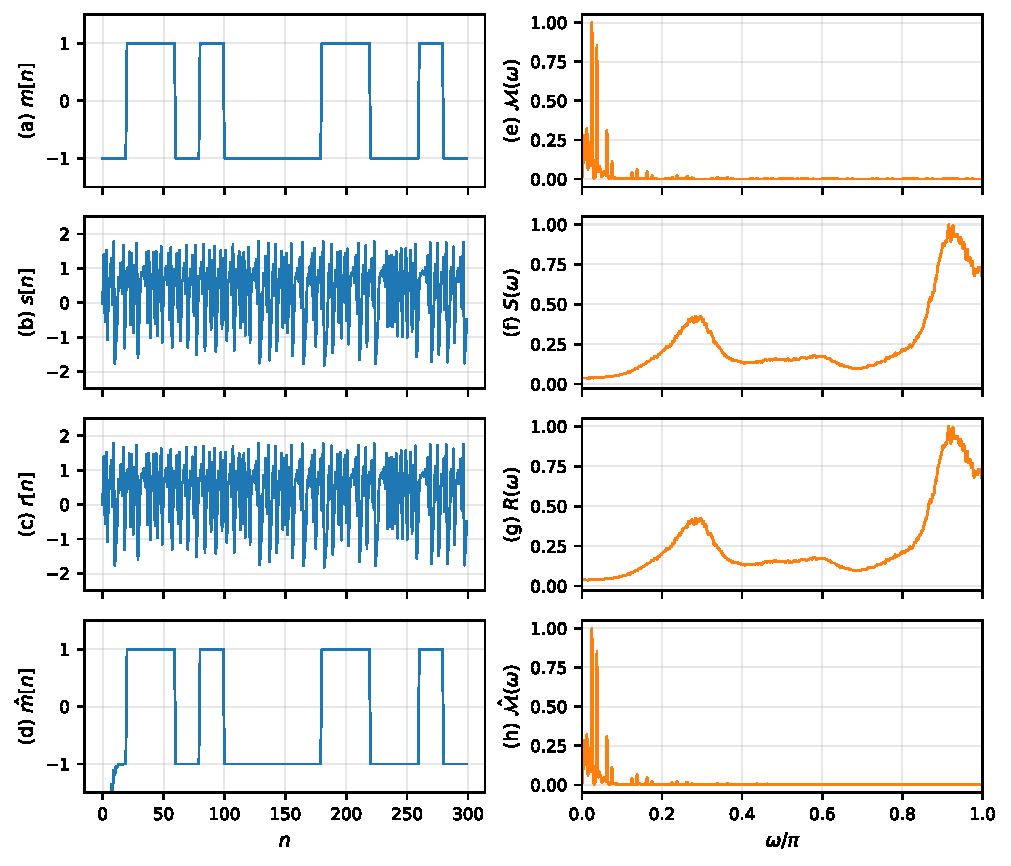
\includegraphics[width=0.88\textwidth]{figures/fig_comm_ideal.pdf}
\label{fig:comm_ideal_pfc}
\end{figura}

A Figura~\ref{fig:comm_fir_pfc} mostra o canal FIR de 201 coeficientes,
janela de Hamming e corte \(0{,}99\pi\). Sem filtro na malha do gerador, a
mensagem recuperada não acompanha a mensagem original: a BER é 0,4324 e o MSE
é 831. Com um filtro de 9 coeficientes, \(N_z=8\), janela de Hamming e corte
\(0{,}52\pi\), a BER cai para zero e o MSE para \(1{,}9\times10^{-5}\). O
maior expoente de Lyapunov do gerador filtrado nessa configuração é 0,0786,
acima do limiar de classificação.

O atraso de grupo do canal é de 100 amostras e é compensado nas métricas. O
canal de 201 coeficientes é um filtro linear de fase aproximadamente linear,
mas remove as frequências mais altas. Sem o filtro na malha, o receptor não
reconstrói a mensagem, e a BER se aproxima de 0,5. Com o filtro na malha, o
gerador e o receptor compartilham a mesma dinâmica filtrada, e a mensagem é
recuperada. A diferença entre os dois casos é qualitativa, não uma melhoria
marginal.

\begin{figura}{Mensagem recuperada e mensagem atrasada em 100 amostras para o
canal FIR de 201 coeficientes, janela de Hamming e corte \(0{,}99\pi\):
(a) sem filtro na malha do gerador, BER \(=0{,}4324\); (b) com filtro de 9
coeficientes, \(N_z=8\), corte \(0{,}52\pi\), BER \(=0\).}{Fonte: Autoria
própria (2026)}
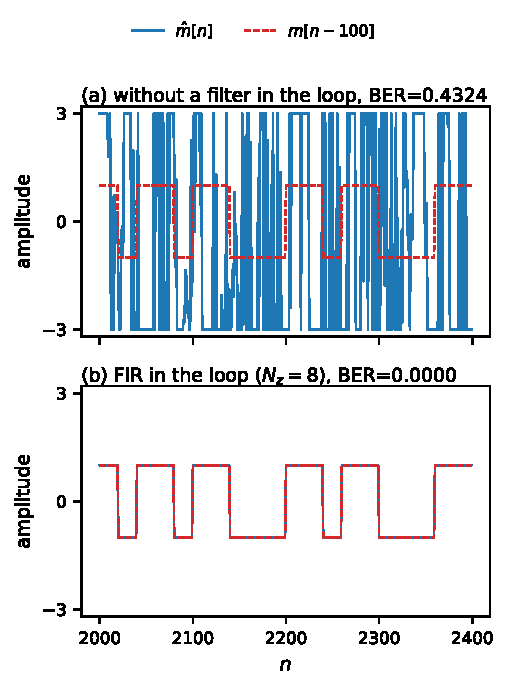
\includegraphics[width=0.50\textwidth]{figures/fig_comm_bandlimited.pdf}
\label{fig:comm_fir_pfc}
\end{figura}

Esses números são uma demonstração de princípio. O canal é linear e conhecido,
o ruído é nulo e a mensagem é um texto curto repetido. O resultado não mede
desempenho em canais com ruído, multicaminho ou desvanecimento, nem compara
o esquema com modulações convencionais. A conclusão defensável é mais
estreita: um filtro no gerador pode tornar o sinal compatível com um canal de
banda limitada sem destruir a sincronização, mas a verificação do caos e a
verificação do enlace são etapas separadas.

\subsection{Robustez, testes e integração contínua}

A suíte de verificação cobre contratos, propriedades, metamorfismo,
regressão numérica, determinismo entre threads e auditoria do manuscrito. Na
execução de referência, o comando de qualidade do repositório terminou com
1.482 testes aprovados, 4 ignorados e 18 deselecionados. A auditoria do JCIS
terminou com 0 erro e 10 avisos. O PFC acrescenta dois scripts próprios: um
confere os números extraídos do PDF contra as fontes calculadas ou medidas, e
outro confere os caminhos e nomes citados nos diagramas.

Os dois exemplos de falha segura são parte do resultado de engenharia. A
auditoria foi tornada \emph{fail-closed}: uma exceção dentro de uma checagem
vira erro, com o nome da checagem e um traceback resumido. O caminho de
figuras e números foi tornado estrito: um checkpoint corrompido interrompe a
execução, e o comportamento tolerante só existe quando solicitado
explicitamente para uso interativo. Esses controles evitam que uma falha
silenciosa produza uma figura ou um número plausível, porém incorreto.

Nem todo tratamento de exceção é fail-closed, e isso é intencional. A sonda de
LaTeX retorna um fallback quando o ambiente não tem LaTeX, sem afetar o
resultado científico. A borda da CLI transforma uma falha esperada em uma
mensagem e um código de saída, mas permite \texttt{--debug} para expor o
traceback. Metadados legados corrompidos são descartados com aviso depois da
verificação de integridade. Essas decisões privilegiam a continuidade do uso
interativo e não o caminho que produz o manuscrito.

O Quadro~\ref{qua:ci_pfc} e a Figura~\ref{fig:ci_pfc} mostram que a CI não
verifica apenas se o código executa. Ela barra estilo, tipos, regressão,
violação de contrato, NaN silencioso, mudança de bits nos checkpoints,
números sem origem, PDF quebrado, dependências vulneráveis, segredos e
workflows inseguros. A segurança do artefato é, portanto, uma propriedade do
processo de desenvolvimento, e não apenas do algoritmo.

\subsection{Síntese e ameaças à validade}

Os resultados sustentam três conclusões de engenharia. Primeiro, o pipeline
é reproduzível: a mesma configuração produz os mesmos checkpoints, as mesmas
classes e as mesmas figuras, e os números do texto são derivados desses
artefatos. Segundo, o desempenho é mensurável e localizado: o ganho de 53,3
vezes vem do kernel compilado, o ganho de 3,58 vezes vem do paralelismo na
carga de 4.000 pontos, e a execução completa leva 575 s no ambiente de teste.
Terceiro, a verificação é fail-closed nos pontos que alimentam o texto, o que
reduz o risco de publicar um resultado silenciosamente errado.

As ameaças à validade são igualmente claras. A classificação é local e
depende de um limiar sobre uma estimativa de tempo finito. Transientes longos
podem ser classificados como caóticos no horizonte das varreduras e mudar de
classe em horizontes maiores. Os filtros realizados não reproduzem
exatamente a máscara nominal, e o ganho DC é uma propriedade da grade
estudada. O desempenho foi medido em um único laptop, com um governador de
frequência específico e uma versão específica das bibliotecas. O sistema de
comunicação foi testado em um canal ideal e em um canal FIR conhecido, sem
ruído, multicaminho ou adversário criptográfico. O esquema de Pecora-Carroll
não fornece confidencialidade nem autenticação.

Essas limitações não anulam a contribuição, mas definem o que ela não é. A
ferramenta não substitui a análise assintótica, não garante segurança
criptográfica e não prova que um filtro será adequado a um canal real. Ela
organiza o projeto, mede o que foi executado, verifica a consistência dos
artefatos e torna explícitas as decisões que, de outra forma, ficariam
escondidas em scripts.

% ============================================================================
\section{Considerações finais}
\label{sec:conclusao}

Este trabalho tratou a caracterização do mapa de Hénon filtrado como um
problema de engenharia, e não apenas como uma experiência numérica. A solução
reúne um modelo dinâmico, um estimador de Lyapunov, uma grade de varredura,
checkpoints versionados, uma camada de análise e uma camada de verificação.
O resultado é uma ferramenta que permite reproduzir os mapas, rastrear cada
número do texto e detectar falhas antes que elas cheguem ao manuscrito.

No plano científico, os resultados confirmam que o ganho DC é uma variável
central. Filtros passa-baixas e rejeita-faixa preservam a componente contínua
e mantêm uma região caótica mais ampla; filtros passa-altas e passa-faixa
removem essa componente e reduzem a região caótica. A melhor cobertura
absoluta ocorre no passa-baixas com Kaiser $\beta_K=17$, seguida pelo
passa-faixa com Kaiser $\beta_K=15{,}5$. Os filtros realizados não reproduzem
exatamente a máscara nominal nas ordens estudadas, e a classificação é local
e dependente do horizonte de integração.

No plano de engenharia, o pipeline completo das 184 varreduras leva 575 s no
i7-8550U com oito threads e parada antecipada. O kernel da varredura é 53,3
vezes mais rápido que o modo Python puro com uma thread, e a carga de 4.000
pontos ganha 3,58 vezes com oito threads em quatro núcleos físicos. As
classes dos 4.000 pontos são idênticas com uma e com oito threads. Apenas o
kernel da varredura é compilado; as demais cargas são NumPy/Python ou SciPy e
permanecem próximas de 1,0. Esses números são específicos do ambiente e estão
registrados nos JSON de medição.

A confiabilidade foi tratada com controles explícitos. A auditoria do
manuscrito é fail-closed, o caminho de figuras e números interrompe em caso de
checkpoint corrompido, as entradas públicas são validadas na borda e a
integração contínua barra regressões, NaN silencioso, dependências vulneráveis
e segredos. As decisões tolerantes que restaram, como a sonda de LaTeX e a
borda da CLI, foram documentadas e justificadas. A segurança do artefato de
software não deve ser confundida com segurança criptográfica do esquema de
comunicação.

As limitações sugerem trabalhos futuros. A grade pode ser estendida para
outras larguras de banda, ordens e parâmetros do mapa; filtros IIR e
estruturas de hardware podem ser avaliados; o enlace pode ser testado com
ruído, multicaminho e canais variantes no tempo; e a classificação pode ser
comparada com estimadores assintóticos e com métodos formais. Também é
possível investigar critérios de projeto que combinem cobertura caótica,
seletividade e ganho DC em uma única função objetivo.

A contribuição final é, portanto, dupla. Do lado científico, o trabalho
organiza o efeito do filtro e da janela no regime caótico. Do lado de
engenharia, ele mostra como transformar esse estudo em uma ferramenta
reprodutível, medida, verificável e consciente dos seus limites.

\imprimirreferencias

\end{document}
